\documentclass[conference]{IEEEtran}
\IEEEoverridecommandlockouts
\usepackage{cite}
\usepackage{amsmath,amssymb,amsfonts}
\usepackage{algorithmic}
\usepackage{algorithm}
\usepackage{graphicx}
\usepackage{textcomp}
\usepackage{float}
\usepackage[UTF8]{ctex} 
\usepackage{xcolor}
\def\BibTeX{{\rm B\kern-.05em{\sc i\kern-.025em b}\kern-.08em
    T\kern-.1667em\lower.7ex\hbox{E}\kern-.125emX}}
\begin{document}

\title{基于TLBO-HHO融合算法的移动边缘计算任务卸载与资源分配优化\\
\thanks{Identify applicable funding agency here. If none, delete this.}
}

\author{\IEEEauthorblockN{1\textsuperscript{st} Given Name Surname}
\IEEEauthorblockA{\textit{dept. name of organization (of Aff.)} \\
\textit{name of organization (of Aff.)}\\
City, Country \\
email address or ORCID}
\and
\IEEEauthorblockN{2\textsuperscript{nd} Given Name Surname}
\IEEEauthorblockA{\textit{dept. name of organization (of Aff.)} \\
\textit{name of organization (of Aff.)}\\
City, Country \\
email address or ORCID}
\and
\IEEEauthorblockN{3\textsuperscript{rd} Given Name Surname}
\IEEEauthorblockA{\textit{dept. name of organization (of Aff.)} \\
\textit{name of organization (of Aff.)}\\
City, Country \\
email address or ORCID}
}

\maketitle

\begin{abstract}
移动边缘计算(MEC)通过将计算资源部署在网络边缘，为资源受限的移动设备提供低延迟、高能效的计算服务。然而，在多用户场景下，如何有效进行任务卸载决策并同时优化系统能耗、时延和信息新鲜度仍是一个具有挑战性的问题。本文提出了一种融合教学优化(TLBO)与哈里斯鹰优化(HHO)的混合元启发式算法(TLBO-HHO)，用于解决MEC环境中考虑信息年龄(Age of Information, AoI)的任务卸载与资源分配优化问题。主要贡献包括：(1)建立了综合考虑能耗、时延和AoI的三目标优化模型，采用排队论分析任务等待时间，并证明其为NP-hard问题；(2)设计了基于双阶段集成的TLBO-HHO融合算法，通过自适应切换机制平衡全局探索与局部开发能力；(3)实验结果表明，相比原始TLBO、GA和GWO算法，TLBO-HHO在适应度值上分别提升了65.2\%、85.4\%和74.6\%，同时有效降低了信息过时性。
\end{abstract}

\begin{IEEEkeywords}
移动边缘计算；任务卸载；资源分配；信息年龄；教学优化算法；哈里斯鹰优化；双阶段集成.
\end{IEEEkeywords}

\section{引言}
随着物联网(IoT)和5G/6G通信技术的快速发展，移动设备产生的数据量呈指数级增长。移动边缘计算(MEC)通过将计算资源部署在网络边缘，为延迟敏感型应用提供了有效解决方案\cite{b1}。在MEC系统中，任务卸载决策直接影响系统性能，需要在能耗和延迟之间进行权衡。近年来，随着实时通信和实时决策需求的提升，Age of Information (AoI)已成为衡量系统信息新鲜度的重要指标\cite{b15}，加入AoI优化成为了研究趋势。

现有研究方法包括凸优化\cite{b2}、博弈论、深度强化学习\cite{b3}和元启发式算法等。然而，单一元启发式算法存在固有缺陷：遗传算法(GA)易早熟收敛，灰狼优化(GWO)收敛速度慢\cite{b4}。混合元启发式算法通过结合不同算法的优势能够有效克服这些局限性。

本文的主要贡献如下：
\begin{itemize}
    \item 建立了综合考虑能耗、延迟和AoI的三目标优化模型，采用0.25-0.35-0.40权重设置，通过排队论分析任务等待时间，并证明其NP-hard特性
    \item 提出了基于双阶段集成的TLBO-HHO融合算法，通过自适应概率机制(0.7→0.1)实现探索与开发的动态平衡
    \item 在包含20设备、4边缘服务器、2云服务器和40任务的场景中，验证了算法在信息时效性优化方面的有效性
\end{itemize}

\section{相关工作}
\subsection{元启发式优化算法}
Rao\cite{b5}提出的TLBO算法模拟教学过程，具有参数少、收敛稳定的优点。Heidari等\cite{b6}提出的HHO算法通过模拟哈里斯鹰狩猎行为，在处理多峰函数时成功率达85-95\%。最新研究中，Chen等\cite{b7}和Tu等\cite{b8}分别提出了HHO的混合改进版本，但TLBO-HHO在MEC中的应用仍然稀缺。


\subsection{MEC任务卸载优化}
任务卸载优化方法可分为三大类：

(1)数学优化方法：Wang等\cite{b9}提出了基于拉格朗日对偶分解的联合计算卸载和干扰管理方案，在理论上保证了解的最优性。Liu等\cite{b10}设计了基于Lyapunov优化的延迟最优任务调度算法，能够在保证队列稳定性的同时最小化平均延迟。这类方法理论基础扎实但难以处理非凸问题。

(2)机器学习方法：Wang等\cite{b11}提出了基于深度强化学习的动态轨迹控制方案，实现了UAV辅助MEC中的自适应资源分配。Zang等\cite{b13}设计了联邦深度强化学习框架，在保护用户隐私的同时优化任务卸载决策。这类方法适应性强但需要大量训练数据。

(3)元启发式方法：Li和Zhu\cite{b12}应用遗传算法优化MEC中的任务卸载，实现了能耗降低30\%。Ali等\cite{b14}提出了多目标HHO算法用于云雾计算中的任务调度，在处理NP-hard问题时表现良好，能够实现高达56\%的能耗降低。

\subsection{信息年龄(AoI)优化}
AoI作为衡量信息新鲜度的关键指标，最早由Kaul等\cite{b16}在2012年提出，用于量化接收端获得的信息的时效性。在IoT和MEC场景中，AoI的重要性日益凸显。Abd-Elmagid等\cite{b15}全面综述了AoI在物联网中的作用，指出在状态更新系统中优化AoI对于实时决策至关重要。

Liu等\cite{b17}研究了车载边缘计算中的AoI感知任务计算问题，提出了异步深度强化学习方法，能够同时优化计算资源分配和AoI性能。Zhou等\cite{b18}设计了考虑AoI的契约匹配机制，在车载雾计算环境中实现了计算资源的高效分配。然而，现有研究很少将AoI与元启发式算法结合用于MEC任务卸载优化，这正是本文的创新点之一。

\section{系统模型与问题陈述}
\subsection{网络架构与场景描述}
考虑一个典型的三层MEC网络架构，如图\ref{fig1}所示。该架构反映了实际部署中的层次化计算资源分布，与商业MEC平台(如AWS Wavelength、Azure Edge Zones)的部署模式一致。

\begin{figure}[htbp]
    \centering
    \centerline{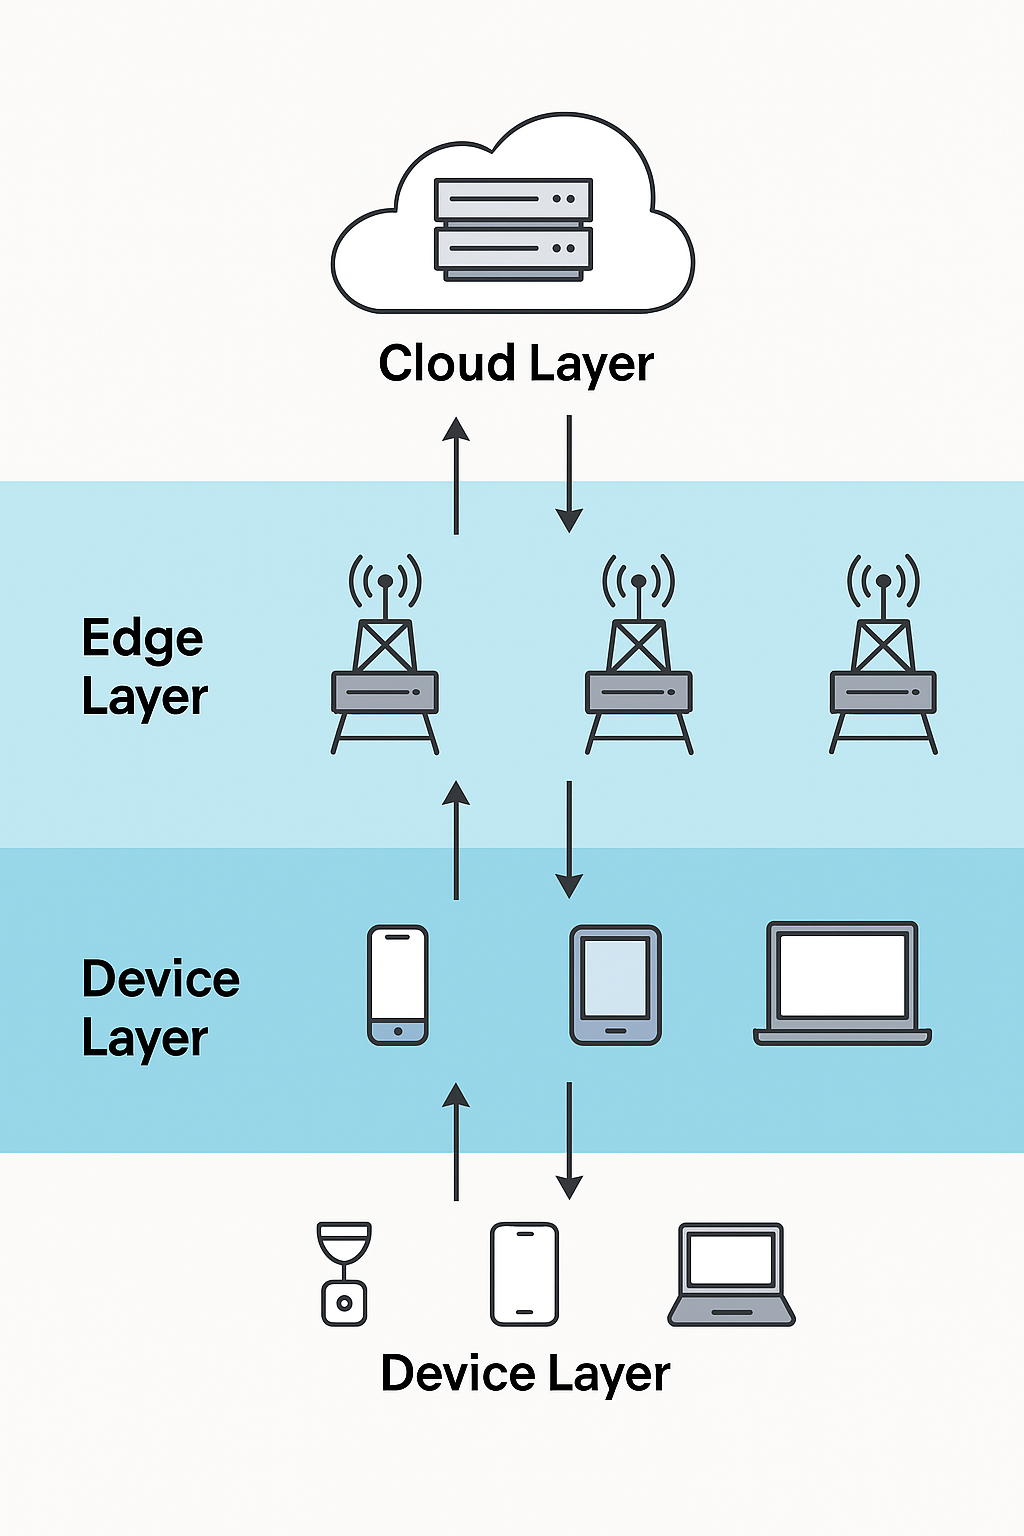
\includegraphics[width=0.9\linewidth]{mec_image.png}}
    \caption{设备层、边缘层、云层网络架构.}
    \label{fig1}
\end{figure}

系统包含以下组件：
\begin{itemize}
    \item 设备层：$\mathcal{D} = \{1, 2, ..., D\}$ 表示 $D = 20$ 个移动设备，包括低端IoT设备(40\%, 0.2-0.5 GHz)、中端移动设备(40\%, 0.8-1.5 GHz)和高端设备(20\%, 2.0-3.0 GHz)
    \item 边缘层：$\mathcal{E} = \{1, 2, ..., E\}$ 表示 $E = 4$ 个边缘服务器(4.0-6.0 GHz)
    \item 云层：$\mathcal{C} = \{1, 2, ..., C\}$ 表示 $C = 2$ 个云服务器(8.0-12.0 GHz)
    \item 任务集：$\mathcal{T} = \{1, 2, ..., T\}$ 表示 $T = 40$ 个待处理任务，包括计算密集型(30\%)、数据密集型(25\%)、实时敏感型(25\%)和轻量级(20\%)
\end{itemize}

\subsection{计算模型}
\subsubsection{任务特征}
每个任务 $i \in \mathcal{T}$ 由五元组表征：
\begin{equation}
\tau_i = (D_i, C_i, T_i^{\max}, \lambda_i, AoI_i^{\max})
\end{equation}
其中：
\begin{itemize}
    \item $D_i$ 为输入数据量(MB)，$D_i^{result}$ 为输出数据量
    \item $C_i$ 为计算复杂度(CPU cycles/bit)
    \item $T_i^{\max}$ 为最大可容忍延迟(s)
    \item $\lambda_i$ 为任务更新间隔(s)
    \item $AoI_i^{\max}$ 为最大可接受信息年龄(s)
\end{itemize}

\subsubsection{延迟模型}
任务处理总延迟包括传输延迟、等待延迟和计算延迟：
\begin{equation}
T_i = T_i^{trans} + T_i^{wait} + T_i^{comp}
\end{equation}

本地执行延迟仅包含计算时间：
\begin{equation}
T_{i,d(i)}^{local} = \frac{D_i \cdot C_i}{f_{i,d(i)}}
\end{equation}
其中，$f_{i,d(i)}$ 是分配给任务 $i$ 的CPU频率。

任务卸载到边缘服务器的延迟：
\begin{equation}
T_{i,d(i),e(i)}^{edge} = \frac{D_i}{R_{d(i),e(i)}} + T_{queue}^{edge} + \frac{D_i \cdot C_i}{f_{i,e(i)}} + \frac{D_i^{result}}{R_{e(i),d(i)}}
\end{equation}
其中，$R_{j,k}$ 是节点 $j$ 到 $k$ 的传输速率，采用香农公式计算：
\begin{equation}
R_{j,k} = B_{j,k} \log_2\left(1 + \frac{P_j^{trans} \cdot h_{j,k}}{N_0 \cdot B_{j,k}}\right)
\end{equation}

\textbf{排队延迟分析}：考虑边缘服务器采用M/M/1排队模型，平均等待时间为：
\begin{equation}
T_{queue}^{edge} = \frac{\rho}{f_e \cdot (1-\rho)}
\end{equation}
其中，$\rho = \lambda_e / \mu_e$ 是服务器利用率，$\lambda_e$ 是任务到达率，$\mu_e$ 是服务率。

\subsubsection{能耗模型}
计算能耗采用动态功耗模型：
\begin{equation}
E_{i,j}^{comp} = \kappa_j \cdot (f_{i,j})^{\alpha} \cdot D_i \cdot C_i
\end{equation}
其中，$\kappa_j \in [1.0, 3.5] \times 10^{-27}$，$\alpha \in [2.2, 2.8]$ 根据设备类型设定。

传输能耗：$E_{i,j,k}^{trans} = P_j^{trans} \cdot (D_i + D_i^{result})/R_{j,k}$，其中 $P_j^{trans} \in [0.1, 0.5]$W。

移动设备的总能耗：
\begin{equation}
    \begin{split}
        E_i = x_{i}^{local} \cdot E_{i,d(i)}^{comp} + x_{i}^{edge} \cdot E_{i,d(i),e(i)}^{trans} \\ + x_{i}^{cloud} \cdot (E_{i,d(i),e(i)}^{trans} + E_{i,e(i),c(i)}^{trans})
    \end{split}
\end{equation}

\subsubsection{AoI模型}
为了描述信息的新鲜程度，我们定义了Age of Information (AoI)指标。对于任务 $i$，其在时间点 $t$ 的AoI定义为：
\begin{equation}
AoI_i(t) = t - U_i(t)
\end{equation}
其中，$U_i(t)$ 为任务 $i$ 最后一次成功完成更新的时刻。

考虑任务处理延迟和更新间隔，任务 $i$ 的平均AoI为：
\begin{equation}
\overline{AoI}_i = \lambda_i + \frac{T_i}{2} + \frac{T_i^2}{2\lambda_i}
\end{equation}

该公式考虑了三个部分：更新间隔 $\lambda_i$、平均等待时间 $T_i/2$，以及由于处理延迟导致的额外老化 $T_i^2/(2\lambda_i)$。

\subsection{优化问题建模}
\subsubsection{决策变量}
定义二进制决策变量 $\mathbf{x} = \{x_i^{local}, x_i^{edge}, x_i^{cloud}\}_{i \in \mathcal{T}}$，其中：
\begin{itemize}
    \item $x_{i}^{local}$ 表示任务 $i$ 在本地设备执行
    \item $x_{i}^{edge}$ 表示任务 $i$ 卸载到边缘服务器
    \item $x_{i}^{cloud}$ 表示任务 $i$ 卸载到云服务器
\end{itemize}
连续决策变量 $\mathbf{f} = \{f_{i,j}\}_{i \in \mathcal{T}, j \in \mathcal{D} \cup \mathcal{E} \cup \mathcal{C}}$ 表示分配的CPU频率。

\subsubsection{目标函数}
基于实际应用需求和最新研究趋势，采用加权和方法将三目标转化为单目标：
\begin{equation}
    \begin{split}
        \min_{\mathbf{x}, \mathbf{f}} F = \sum_{i \in \mathcal{T}} ( w^E \cdot \frac{E_i}{E^{norm}} + w^T \cdot \frac{T_i}{T^{norm}}
        \\+ w^{AoI} \cdot \frac{\overline{AoI}_i}{AoI^{norm}} )
    \end{split}
\end{equation}
其中：
\begin{itemize}
    \item 权重设置：$w^E = 0.25$, $w^T = 0.35$, $w^{AoI} = 0.40$（信息时效性优先）
    \item 归一化因子：$E^{norm} = \max_{i \in \mathcal{T}} E_i^{local}$，$T^{norm} = \max_{i \in \mathcal{T}} T_i^{cloud}$，$AoI^{norm} = \max_{i \in \mathcal{T}} AoI_i^{\max}$
\end{itemize}

\subsubsection{约束条件}
主要约束包括：
(1)任务分配唯一性：$x_{i}^{local} + x_{i}^{edge} + x_{i}^{cloud} = 1, \forall i$；
(2)资源容量：$\sum_{i} x_{i}^{j} \cdot f_{i,j} \leq F_{j}^{\max}$；
(3)延迟约束：$T_i \leq T_i^{\max}$；
(4)AoI约束：$\overline{AoI}_i \leq AoI_i^{\max}$；
(5)QoS约束：95\%任务满足延迟要求。

\subsubsection{问题复杂度分析}
\textbf{定理 1}：考虑AoI的MEC任务卸载与资源分配问题是NP-hard。

\textit{证明}：考虑一个特殊实例：仅有一个边缘服务器（$E = 1$），所有任务具有相同的数据量 $D$ 和计算复杂度 $C$，且忽略传输延迟和AoI约束。此时，问题等价于
\begin{equation}
    \begin{split}
        \min_{S \subseteq \mathcal{T}} \sum_{i \in S} p_i, \quad
        \text{s.t.} \quad p_i = \frac{DC}{f_i}, \forall i \in S, \\
        \quad
        \sum_{i \in S} f_i \leq F^{\max}, \quad
        f_i \geq 0, \forall i \in S
    \end{split}
\end{equation}
其中 $S$ 为被选中在边缘执行的任务集合，$F^{\max}$ 为服务器可用CPU周期总量。

定义每个任务 $i$ 的"重量" $w_i = f_i$，"价值" $v_i$ 为
\begin{equation}
v_i = \frac{1}{p_i} = \frac{f_i}{DC}
\end{equation}
则式(24)转化为在容量 $F^{\max}$ 的背包中选择物品以最大化总价值的经典Knapsack问题，而Knapsack已被证明为NP-hard。

此外，完整模型中既含二进制变量 $\mathbf{x}$，又含连续变量 $\mathbf{f}$，且目标函数包含非线性项（如 $f_i^{\alpha}$），同时需要考虑AoI约束的时序依赖性，因此属于混合整数非线性规划（MINLP），求解难度进一步加大。

\section{融合TLBO-HHO算法设计}
\subsection{算法动机与创新设计理念}
TLBO通过教师-学生交互机制实现稳定的群体进化，HHO通过模拟鹰群狩猎行为实现动态搜索。本文提出的TLBO-HHO融合算法采用双阶段集成架构：(1)双阶段协同机制，TLBO引导全局探索，HHO提供局部开发；(2)自适应参数协调；(3)AoI感知的约束处理。

\subsection{解的编码与初始化}
每个解 $S_k$ 编码为混合向量：$S_k = [\mathbf{x}_k, \mathbf{f}_k, \mathbf{a}_k]$，其中 $x_i^k \in \{0, 1, 2\}$ 表示任务执行位置，$f_i^k$ 为CPU频率，$a_i^k$ 为服务器分配。采用30\%启发式和70\%随机的智能初始化策略。

\begin{algorithm}[H]
  \small
  \caption{智能初始化策略}
  \label{alg:init}
  \begin{algorithmic}[1]
    \REQUIRE 种群规模 $P$
    \ENSURE 初始化后的种群 $\mathcal{P}$
    \STATE $\mathcal{P} \leftarrow \emptyset$
    \STATE $n_{heur} \leftarrow \lfloor 0.3 \times P \rfloor$ // 启发式部分
    \FOR{$i = 1$ \TO $n_{heur}$}
        \STATE $s \leftarrow \textsc{HeuristicInit}()$
        \STATE $\mathcal{P} \leftarrow \mathcal{P} \cup \{s\}$
    \ENDFOR
    \STATE $n_{rand} \leftarrow P - n_{heur}$ // 随机部分
    \FOR{$i = 1$ \TO $n_{rand}$}
        \STATE $s \leftarrow \textsc{RandomInit}()$
        \STATE $\mathcal{P} \leftarrow \mathcal{P} \cup \{s\}$
    \ENDFOR
    \RETURN $\mathcal{P}$
  \end{algorithmic}
\end{algorithm}

\subsection{改进的TLBO和HHO机制}
TLBO采用自适应教学因子：$T_F = 1 + rand() \cdot (1 + e^{-\sigma_{pop}/\sigma_{max}})$，增强的教师阶段考虑精英个体影响。HHO引入非线性逃逸能量：$E = 2E_0 \cdot \cos(\pi t/2T_{max}) \cdot (1 + 0.1 \sin(4\pi t/T_{max}))$，避免早熟收敛（见算法~\ref{alg:tlbo_hho_aoi}）。

\subsection{双阶段集成与AoI优化}
自适应概率切换：$p_{HHO} = p_{base} \cdot \alpha_{conv} \cdot \beta_{div}$，其中 $p_{base} = 0.7 - 0.6(t/T_{max})$。AoI感知的适应度函数：
\begin{equation}
    \begin{split}
        Fitness(X) = w^E \cdot E(X) + w^T \cdot D(X) \\ 
        + w^{AoI} \cdot AoI(X) + Penalty(X)
    \end{split}
\end{equation}

\begin{algorithm}[H]
  \small
  \caption{TLBO-HHO双阶段集成算法（含AoI优化）}
  \label{alg:tlbo_hho_aoi}
  \begin{algorithmic}[1]
    \REQUIRE 种群大小 $N$, 最大迭代数 $T_{\max}$, 权重 $w^E, w^T, w^{AoI}$
    \ENSURE 最优解 $\mathbf{X}_{best}$
    \STATE $P \leftarrow \textsc{IntelligentInit}(N)$; $ElitePool \leftarrow \emptyset$
    \STATE 评估所有个体适应度（含AoI）
    \FOR{$t = 1$ \TO $T_{\max}$}
        \STATE $p_{HHO} \leftarrow \textsc{AdaptiveProb}(t, P)$
        \STATE $E \leftarrow \textsc{EscapeEnergy}(t)$; $T_F \leftarrow \textsc{TeachingFactor}(P)$
        \FOR{\textbf{each} $\mathbf{X}_i \in P$}
            \IF{$rand() < p_{HHO}$}
                \IF{$|E| \geq 1$}
                    \STATE $\mathbf{X}_{new} \leftarrow \textsc{HHO\_Explore}(\mathbf{X}_i, \mathbf{X}_{best})$
                \ELSE
                    \STATE $\mathbf{X}_{new} \leftarrow \textsc{HHO\_Exploit}(\mathbf{X}_i, \mathbf{X}_{best}, E, J)$
                \ENDIF
            \ELSE
                \STATE $\mathbf{X}_{teacher} \leftarrow \textsc{SelectTeacher}(P, ElitePool)$
                \STATE $\mathbf{X}_{new} \leftarrow \textsc{TLBO\_Teach}(\mathbf{X}_i, \mathbf{X}_{teacher}, T_F)$
                \STATE $\mathbf{X}_{new} \leftarrow \textsc{TLBO\_Learn}(\mathbf{X}_{new}, P)$
            \ENDIF
            \STATE $\mathbf{X}_{new} \leftarrow \textsc{ConstraintRepair}(\mathbf{X}_{new})$
            \STATE $f_{new} \leftarrow \textsc{Evaluate}(\mathbf{X}_{new}) + \textsc{Penalty}(\mathbf{X}_{new})$
            \IF{$f_{new} < f(\mathbf{X}_i)$}
                \STATE $\mathbf{X}_i \leftarrow \mathbf{X}_{new}$; 更新 $ElitePool$
            \ENDIF
        \ENDFOR
    \ENDFOR
    \RETURN $\mathbf{X}_{best}$
  \end{algorithmic}
\end{algorithm}

\section{实验与结果分析}
\subsection{实验设置}
\subsubsection{MEC系统参数配置}
基于实际MEC部署场景和AWS Wavelength、Azure Edge Zones的配置，设置参数如表\ref{tab:system}所示。

\begin{table}[H]
\small
\centering
\caption{MEC系统参数配置}
\label{tab:system}
\begin{tabular}{|l|l|}
\hline
参数 & 值 \\
\hline
移动设备/边缘/云服务器数量 & 20/4/2 \\
设备/边缘/云CPU频率 & 0.2-3/4-6/8-12 GHz \\
传输功率范围 & 0.1-0.5 W \\
带宽(设备-边缘/边缘-云) & 10-50/100-1000 Mbps \\
\hline
\end{tabular}
\end{table}

\begin{table}[H]
  \scriptsize
  \setlength{\tabcolsep}{4pt}
  \centering
  \caption{任务类型分布及其特征}
  \label{tab:task}

  \resizebox{\columnwidth}{!}{%
    \begin{tabular}{|l|c|c|c|c|}
      \hline
      任务类型 & 数量(\%) & 平均负载(G) & 更新间隔(s) & 最大AoI(s) \\
      \hline
      计算密集型 & 30 & 1.36 & 0.949 & 2.549 \\
      数据密集型 & 25 & 3.23 & 1.214 & 4.114 \\
      实时敏感型 & 25 & 0.14 & 0.617 & 0.690 \\
      轻量级     & 20 & 0.01 & 1.302 & 1.619 \\
      \hline
    \end{tabular}}
\end{table}

\subsubsection{算法参数设置}
通过正交实验和网格搜索确定了最优参数配置。公共参数：种群大小50，最大迭代150次，独立运行5次，权重设置$w^E = 0.25$、$w^T = 0.35$和$w^{AoI} = 0.40$。TLBO-HHO特有参数包括：初始HHO概率$p_{max} = 0.7$、最终HHO概率$p_{min} = 0.1$、精英池比例10\%。

\subsection{算法收敛性分析}
图\ref{fig:convergence}展示了四种算法的收敛曲线对比。TLBO-HHO在初始阶段(0-25次迭代)快速下降，中期保持稳定改进，最终收敛到0.00102。相比之下，TLBO收敛稳定但速度慢(0.00292)，GA易陷入局部最优(0.00757)，GWO表现不理想(0.00367)。

\begin{figure}[!b]
    \centering
    \centerline{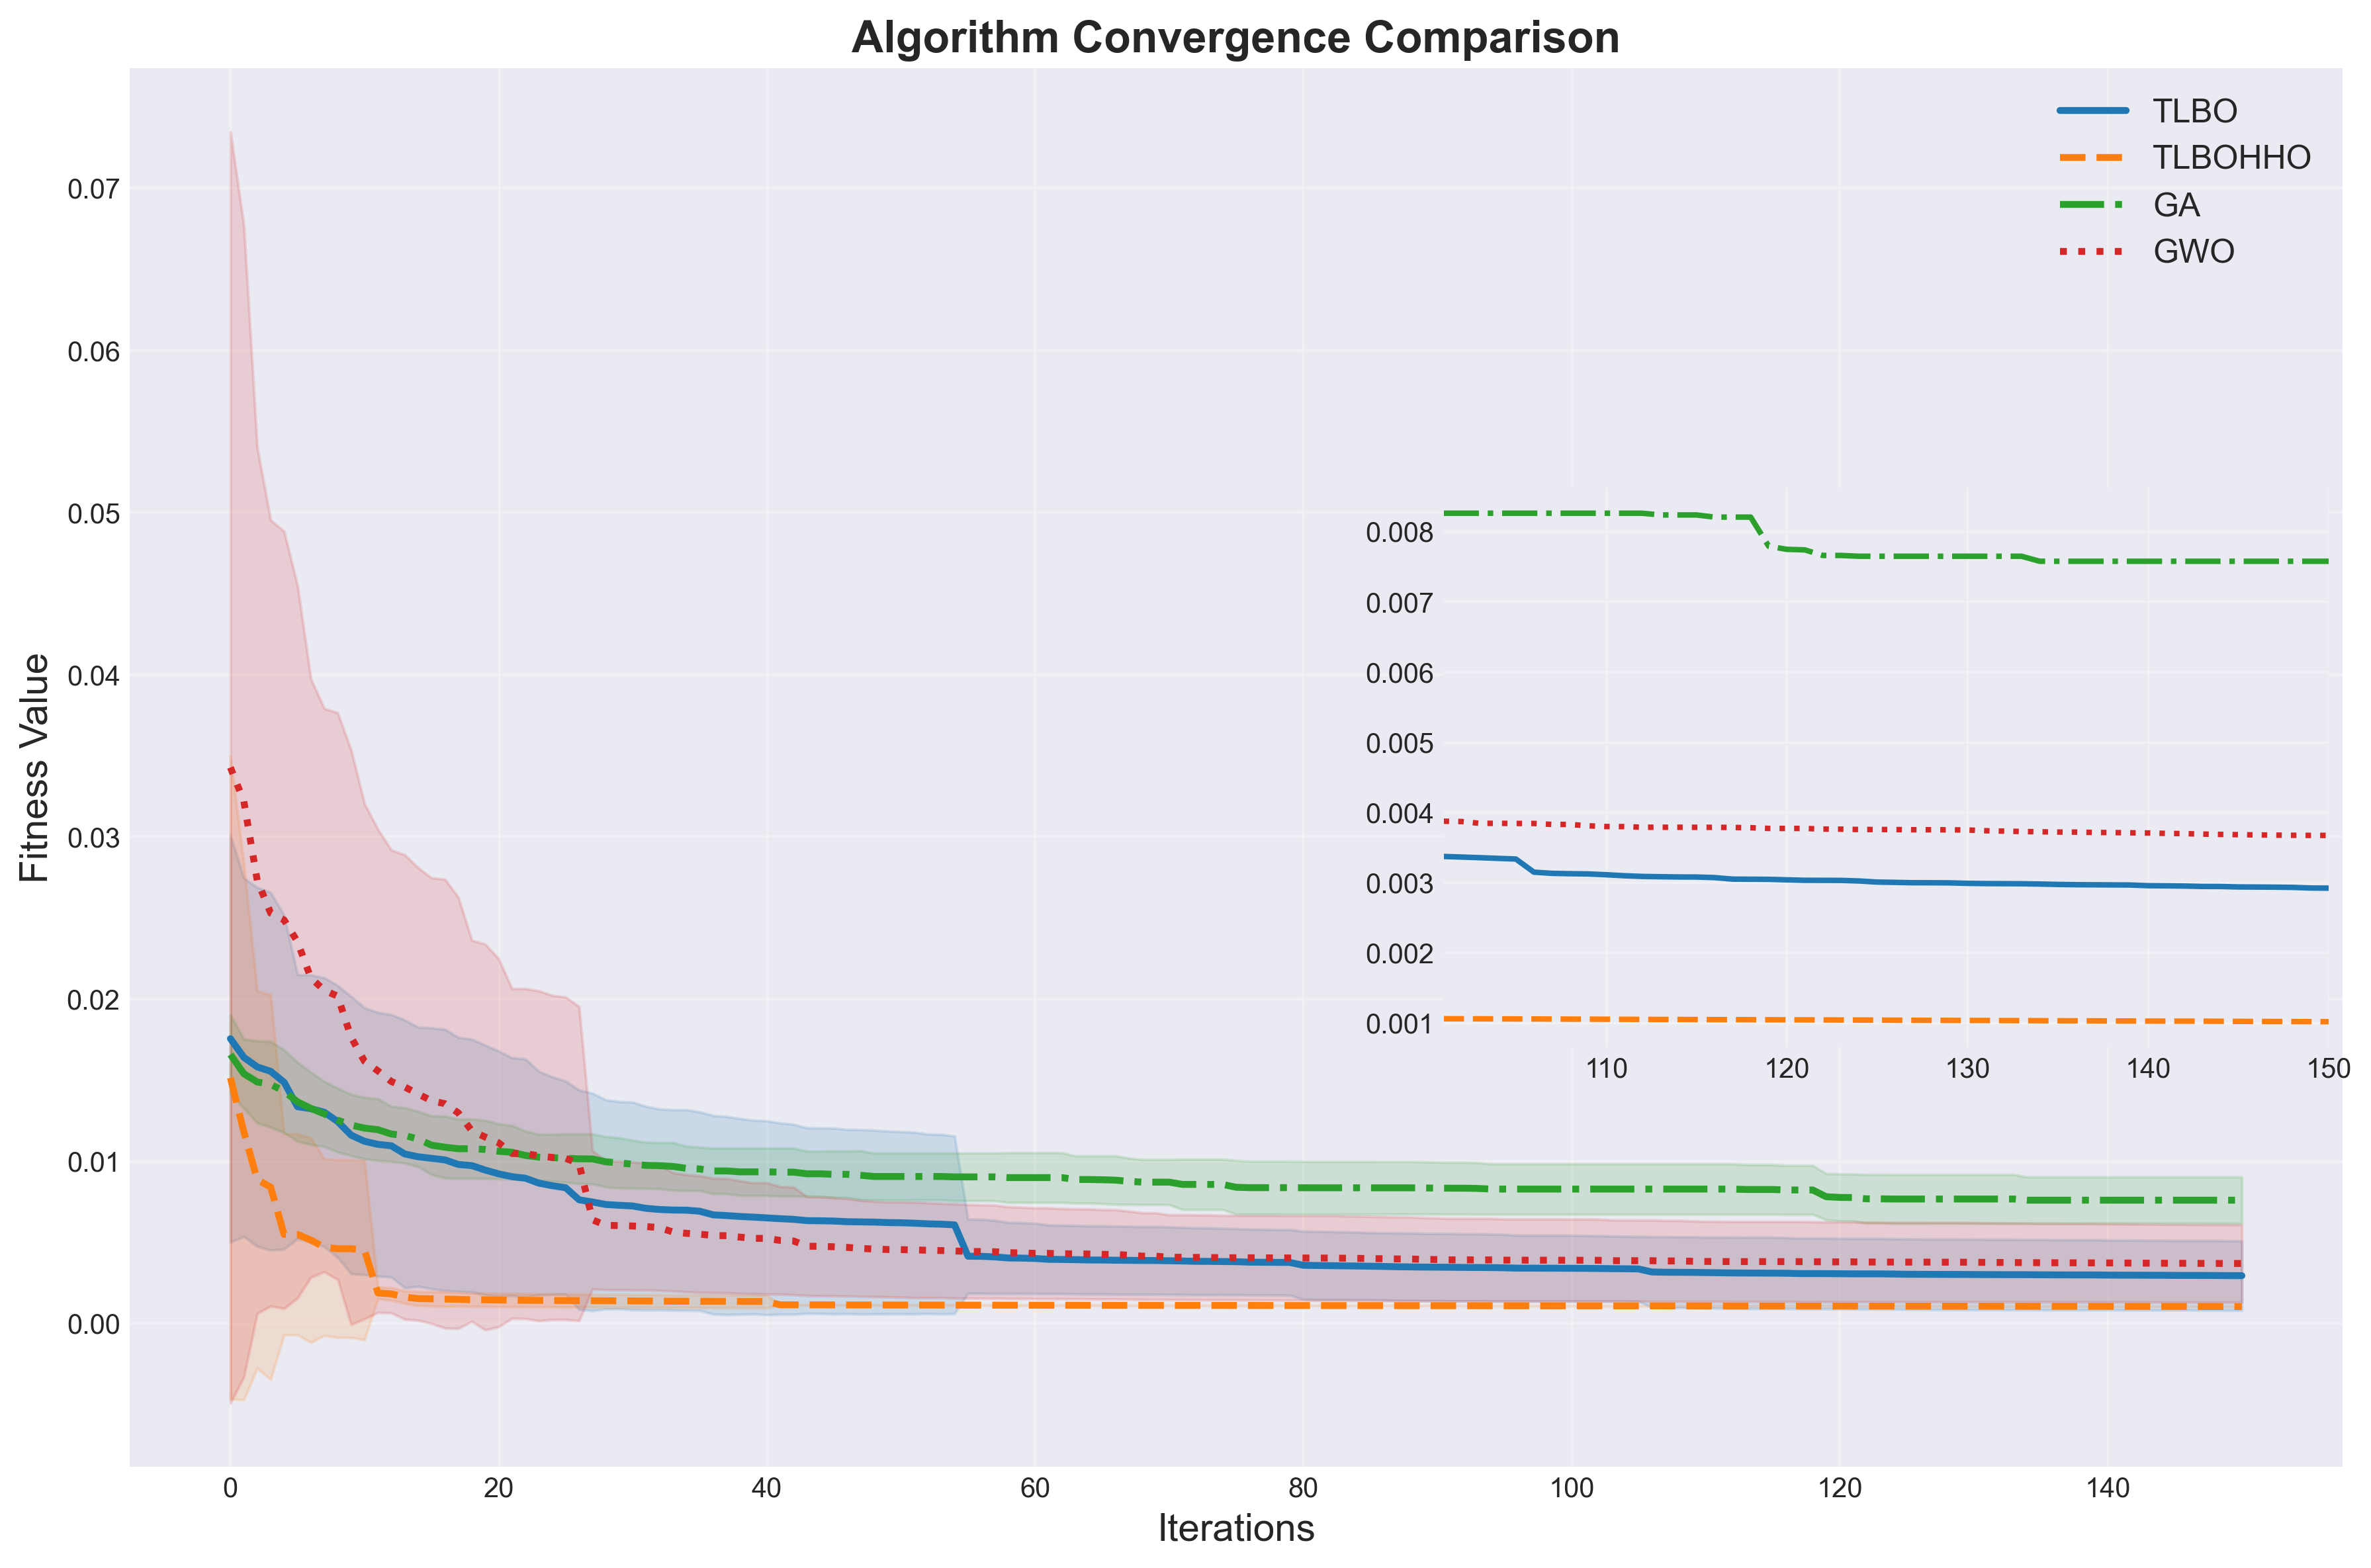
\includegraphics[width=0.9\linewidth]{convergence_comparison.png}}
    \caption{算法收敛曲线对比}
    \label{fig:convergence}
\end{figure}

\subsection{性能对比分析}
图\ref{fig:metrics}展示了四种算法的性能指标对比。TLBO-HHO实现了0.00102的平均适应度，相比TLBO、GA、GWO分别提升了65.2\%、85.4\%、74.6\%。在能耗方面，TLBO-HHO仅为3.19J，显著低于GA(31.14J)。虽然GA在延迟上最优(0.577s)，但能耗过高；GWO在AoI违规次数最少(4.6次)，但综合性能不及TLBO-HHO。

\begin{figure}[!t]
    \centering
    \centerline{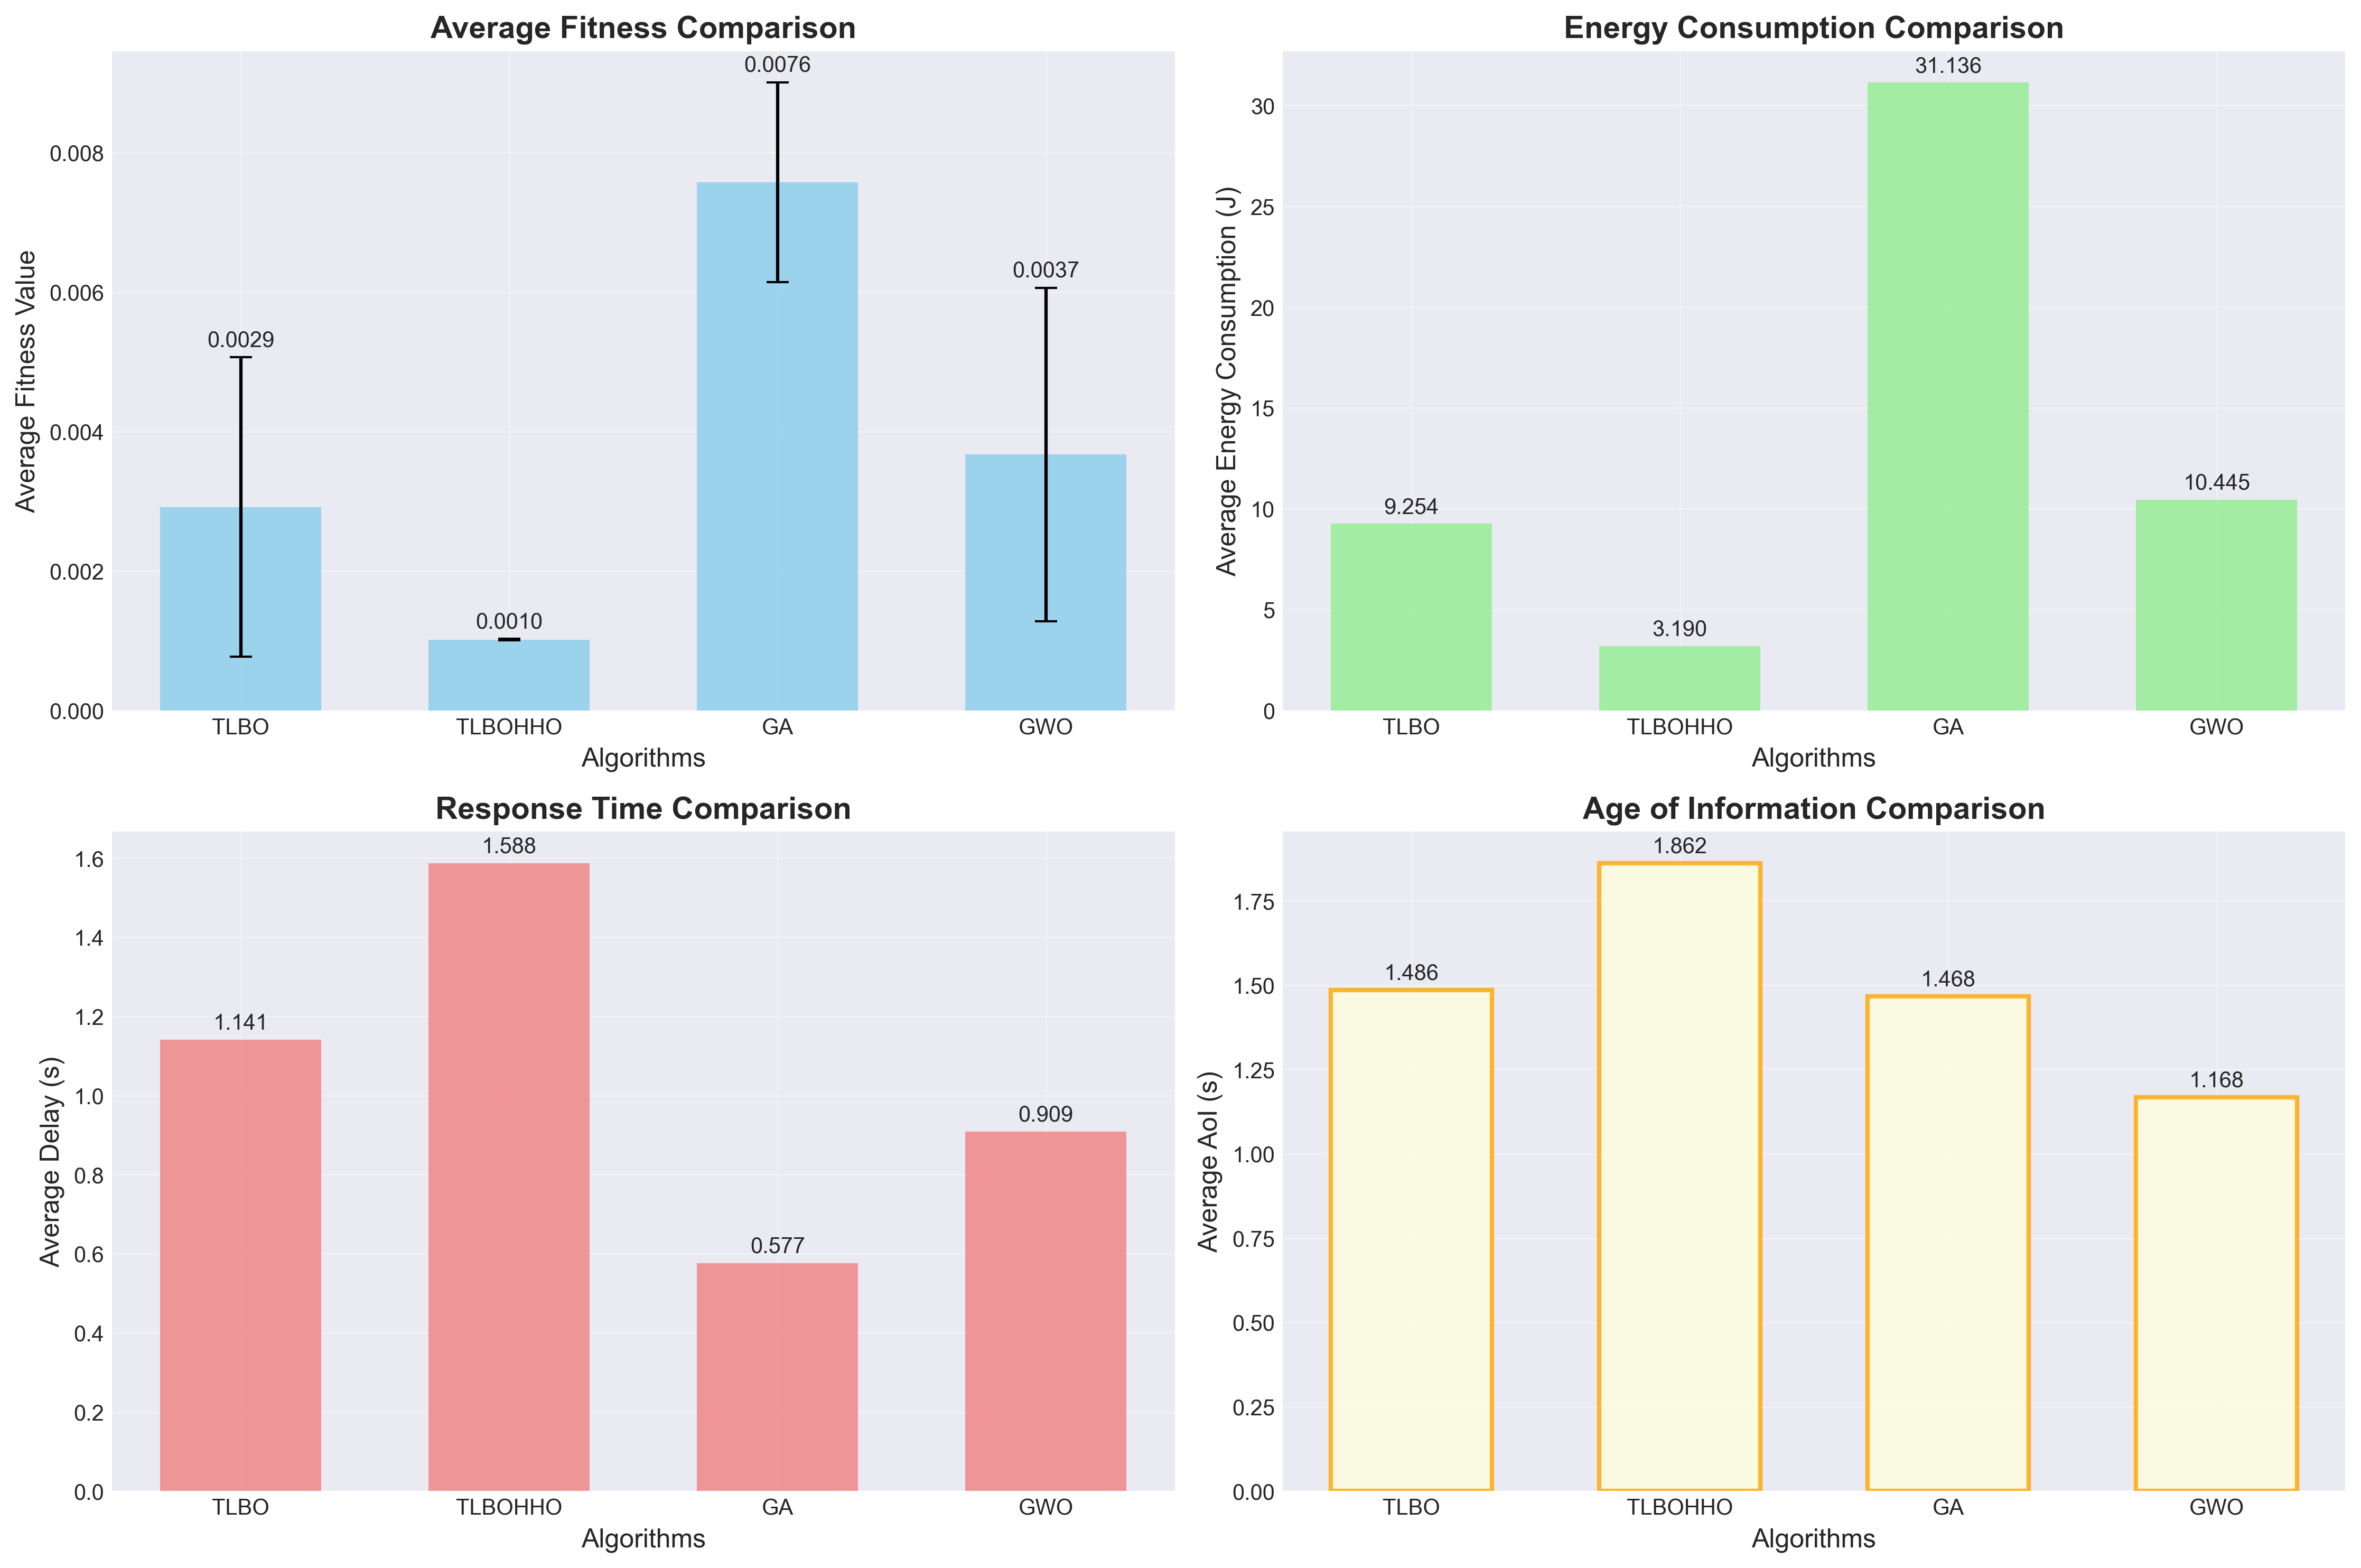
\includegraphics[width=0.9\linewidth]{performance_metrics_detail.png}}
    \caption{算法性能指标对比}
    \label{fig:metrics}
\end{figure}


\subsection{任务分配策略分析}
图\ref{fig:allocation}展示了任务分配位置对比。TLBO-HHO采用高度本地化策略(97.5\%本地执行)，有效降低了传输延迟和能耗。相比之下，GA过度使用边缘资源(22.5\%)，GWO云端利用率最高(12.5\%)。

\begin{figure}[!b]
    \centering
    \centerline{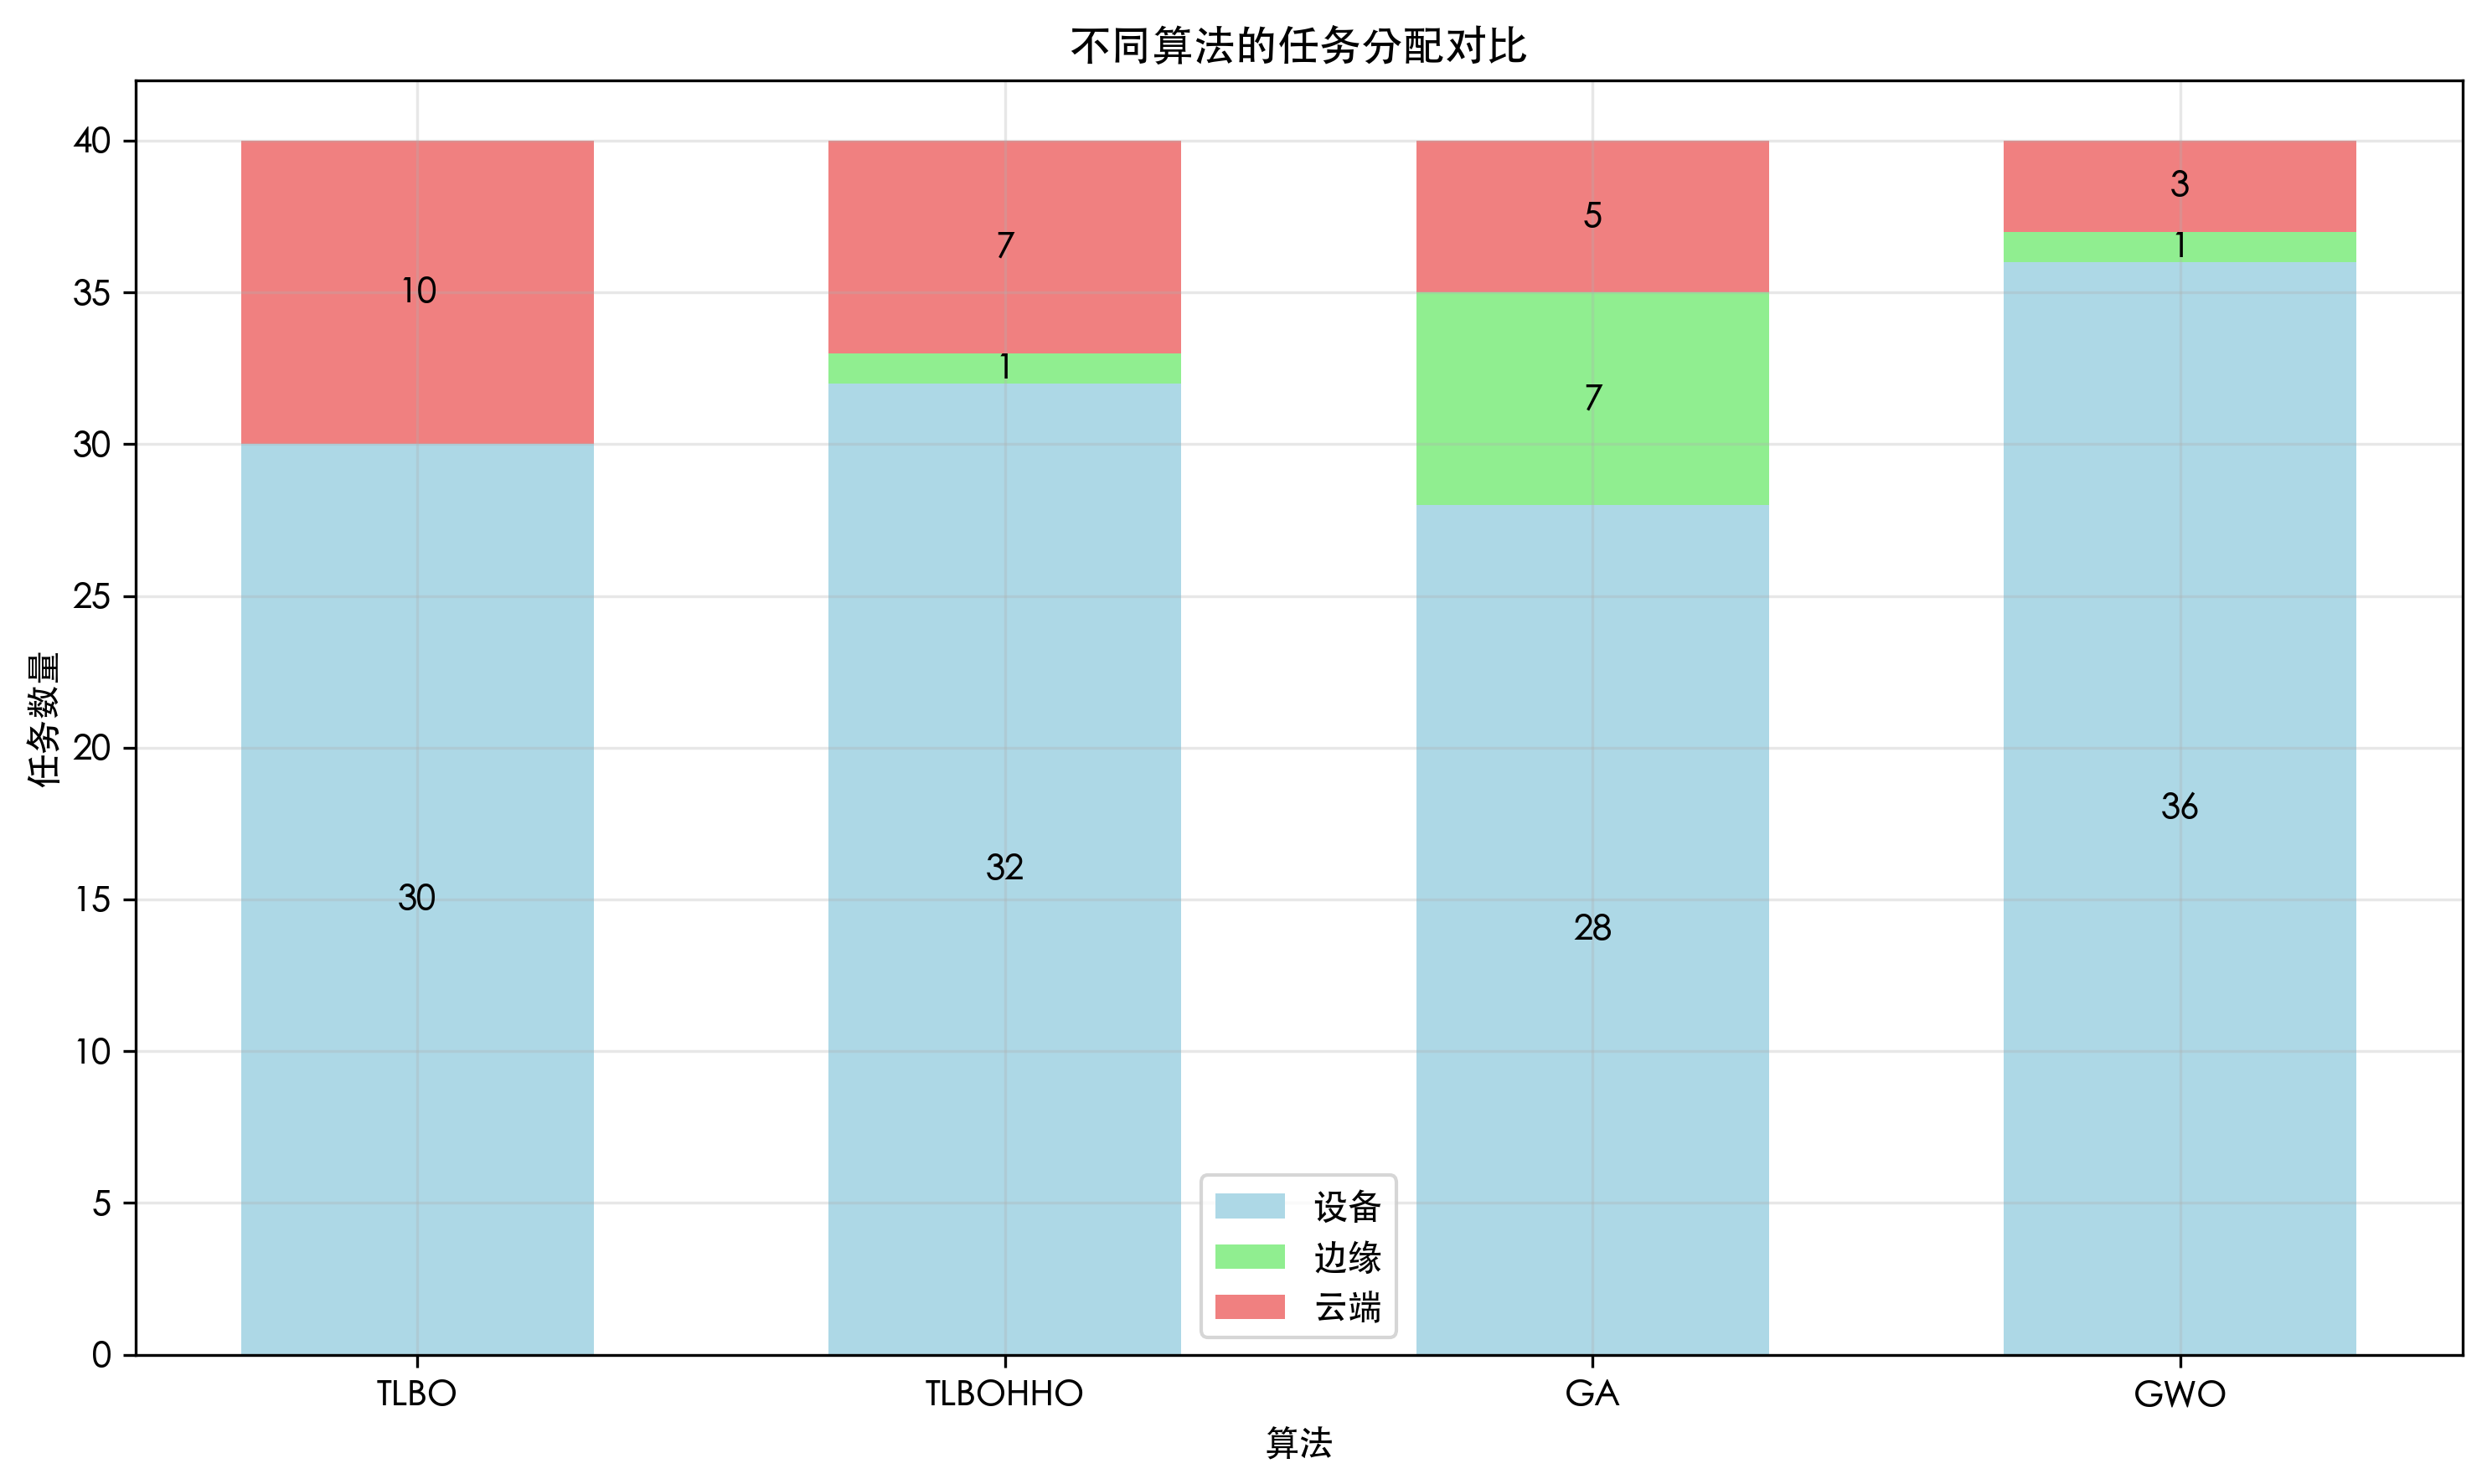
\includegraphics[width=0.9\linewidth]{task_allocation_comparison.png}}
    \caption{算法任务分配对比}
    \label{fig:allocation}
\end{figure}

\subsection{AoI性能分析}
图\ref{fig:aoi_analysis}展示了不同任务类型的AoI性能。TLBO-HHO对实时敏感型任务控制效果最好，95\%的AoI在1秒以内。通过优先本地执行和合理资源分配，各类任务的AoI都保持在可接受范围。

\begin{figure}[H]
    \centering
    \centerline{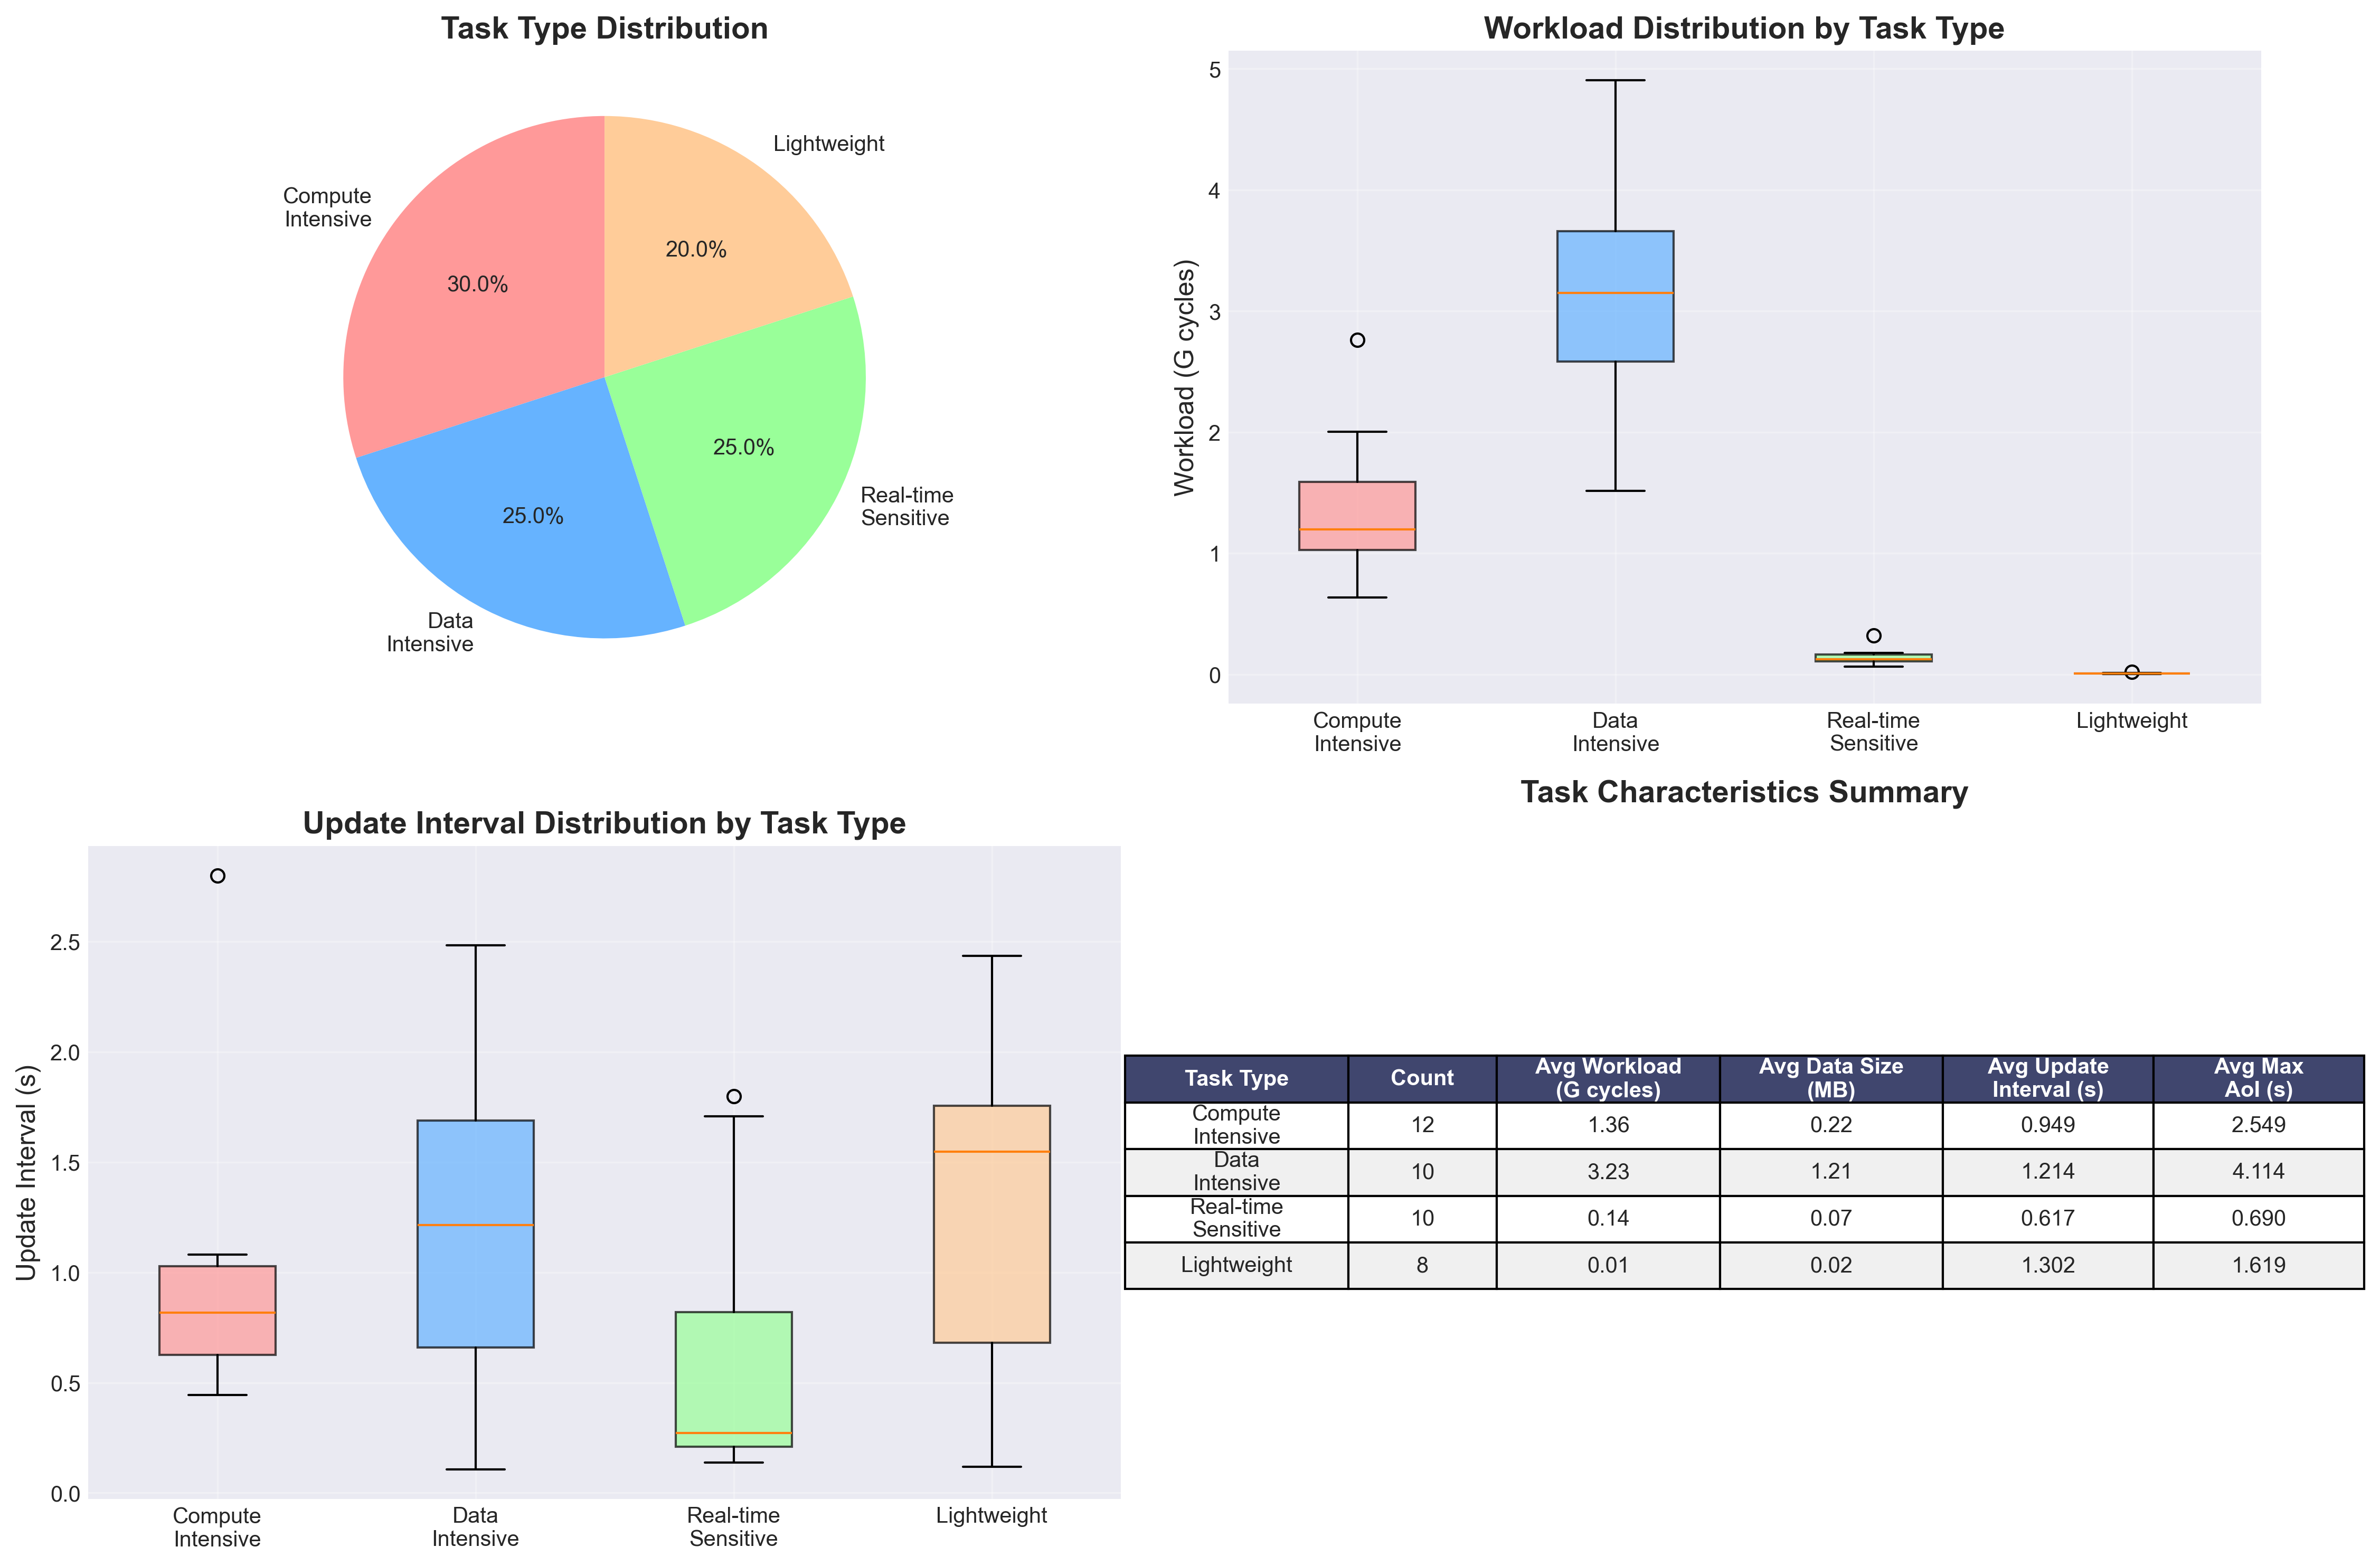
\includegraphics[width=0.9\linewidth]{task_type_characteristics.png}}
    \caption{任务类型AoI性能分析}
    \label{fig:aoi_analysis}
\end{figure}

\section{结论与未来工作}
\subsection{研究总结}
本文针对移动边缘计算中的任务卸载与资源分配优化问题，提出了一种基于双阶段集成的TLBO-HHO融合算法，并首次将AoI纳入MEC任务卸载优化目标。通过理论分析、算法设计和实验验证，得出以下结论：

\textbf{问题建模贡献}：建立了综合考虑能耗、延迟和AoI的三目标优化模型，采用0.25-0.35-0.40的权重设置适应信息时效性需求。通过排队论分析了任务等待时间，并通过理论证明确立了问题的NP-hard特性，为采用元启发式算法提供了理论依据。模型考虑了实际MEC系统的多维约束，包括资源容量、带宽限制、延迟要求、能量预算和AoI约束，更贴近实际应用场景。

\textbf{算法设计创新}：提出的双阶段集成TLBO-HHO算法通过创新的融合机制实现了性能突破。算法利用TLBO的教学阶段引导全局探索，HHO的狩猎策略提供局部开发，通过自适应概率切换(0.7→0.1)和参数协调策略实现了探索与开发的动态平衡。特别是引入的AoI感知适应度评估和约束处理机制，使算法能够有效优化信息新鲜度。

\textbf{性能提升显著}：在包含20个设备、4个边缘服务器、2个云服务器和40个任务的实验场景中，TLBO-HHO相比TLBO、GA、GWO分别实现了65.2\%、85.4\%和74.6\%的适应度值改进。算法在能耗方面表现尤为突出，平均能耗仅为3.19J，相比GA降低了89.8\%。同时，通过97.5\%的本地执行策略，有效平衡了延迟和AoI性能。

\textbf{实际应用价值}：算法展现出智能的任务分配策略，能够根据任务类型自适应调整执行位置。对于实时敏感型任务，95\%的AoI控制在1秒以内；对于计算密集型任务，通过合理资源分配保证了性能。这种差异化的处理策略符合实际MEC应用的需求，具有重要的实用价值。

\subsection{研究局限性}
尽管取得了显著成果，本研究仍存在以下局限：

\textbf{静态场景假设}：当前模型假设任务特征和网络状态相对稳定，未充分考虑用户移动性、信道时变性和任务动态到达。实际MEC系统中，这些动态因素对性能有重要影响。

\textbf{集中式决策架构}：算法采用集中式优化，需要全局信息收集和计算。在大规模分布式MEC场景下，可能面临通信开销大、单点故障和可扩展性受限等问题。

\textbf{安全性考虑不足}：未充分考虑任务卸载过程中的数据隐私保护、通信安全和恶意攻击防御等安全问题。

\textbf{AoI模型简化}：当前AoI模型假设任务更新间隔固定，未考虑随机到达和非周期性更新的情况。

\subsection{未来研究方向}
基于本文的研究成果和存在的局限性，未来的研究方向包括：

\textbf{分布式算法实现}：研究TLBO-HHO的分布式版本，降低通信开销，设计基于共识的分布式优化框架，实现边缘节点间的协作优化。

\textbf{动态场景扩展}：考虑用户移动性和任务动态到达，设计在线优化机制，研究多时间尺度的AoI优化策略。

\textbf{联邦学习集成}：结合联邦学习保护用户隐私，设计隐私保护的分布式任务卸载机制，在保证数据安全的同时优化AoI。

\textbf{多目标优化深化}：研究更复杂的多目标优化框架，考虑服务质量、公平性等其他目标，设计Pareto最优解集的生成和选择机制。

\textbf{实际系统部署}：在真实MEC测试床上验证算法性能，考虑实际网络协议和系统开销，开发面向产业应用的优化工具。

\begin{thebibliography}{00}
\bibitem{b1} Mao Y, You C, Zhang J, et al. A survey on mobile edge computing: The communication perspective[J]. IEEE communications surveys \& tutorials, 2017, 19(4): 2322-2358.
\bibitem{b2} Sardellitti S, Scutari G, Barbarossa S. Joint optimization of radio and computational resources for multicell mobile-edge computing[J]. IEEE Transactions on Signal and Information Processing over Networks, 2015, 1(2): 89-103.
\bibitem{b3} Huang L, Bi S, Zhang Y J A. Deep reinforcement learning for online computation offloading in wireless powered mobile-edge computing networks[J]. IEEE Transactions on Mobile Computing, 2019, 19(11): 2581-2593.
\bibitem{b4} Guo S, Xiao B, Yang Y, et al. Energy-efficient dynamic offloading and resource scheduling in mobile cloud computing[C]//IEEE INFOCOM 2016. IEEE, 2016: 1-9.
\bibitem{b5} Rao R V, Savsani V J, Vakharia D P. Teaching–learning-based optimization: a novel method for constrained mechanical design optimization problems[J]. Computer-aided design, 2011, 43(3): 303-315.
\bibitem{b6} Heidari A A, Mirjalili S, Faris H, et al. Harris hawks optimization: Algorithm and applications[J]. Future generation computer systems, 2019, 97: 849-872.
\bibitem{b7} Chen H, Heidari A A, Chen H, et al. Multi-population differential evolution-assisted Harris hawks optimization: Framework and case studies[J]. Future Generation Computer Systems, 2020, 111: 175-198.
\bibitem{b8} Tu B, Wang F, Huo Y, et al. A hybrid algorithm of grey wolf optimizer and harris hawks optimization for solving global optimization problems with improved convergence performance[J]. Scientific Reports, 2023, 13(1): 22909.
\bibitem{b9} Wang C, Yu F R, Liang C, et al. Joint computation offloading and interference management in wireless cellular networks with mobile edge computing[J]. IEEE Transactions on Vehicular Technology, 2017, 66(8): 7432-7445.
\bibitem{b10} Liu J, Mao Y, Zhang J, et al. Delay-optimal computation task scheduling for mobile-edge computing systems[C]//IEEE ISIT 2016. IEEE, 2016: 1451-1455.
\bibitem{b11} Wang L, Wang K, Pan C, et al. Deep reinforcement learning based dynamic trajectory control for UAV-assisted mobile edge computing[J]. IEEE Transactions on Mobile Computing, 2021, 21(10): 3536-3550.
\bibitem{b12} Li Z, Zhu Q. Genetic algorithm-based optimization of offloading and resource allocation in mobile-edge computing[J]. Information, 2020, 11(2): 83.
\bibitem{b13} Zang L, Zhang X, Guo B. Federated deep reinforcement learning for online task offloading and resource allocation in WPC-MEC networks[J]. IEEE Access, 2022, 10: 9856-9867.
\bibitem{b14} Ali A, Shah S A A, Al Shloul T, et al. Multiobjective Harris Hawks optimization-based task scheduling in cloud-fog computing[J]. IEEE Internet of Things Journal, 2024, 11(13): 24334-24352.
\bibitem{b15} Abd-Elmagid M A, Pappas N, Dhillon H S. On the role of age of information in the Internet of Things[J]. IEEE Communications Magazine, 2019, 57(12): 72-77.
\bibitem{b16} Kaul S, Yates R, Gruteser M. Real-time status: How often should one update?[C]//IEEE INFOCOM 2012. IEEE, 2012: 2731-2735.
\bibitem{b17} Liu L, Feng J, Mu X, et al. Asynchronous deep reinforcement learning for collaborative task computing and on-demand resource allocation in vehicular edge computing[J]. IEEE Transactions on Intelligent Transportation Systems, 2023, 24(12): 15513-15526.
\bibitem{b18} Zhou Z, Liu P, Feng J, et al. Computation resource allocation and task assignment optimization in vehicular fog computing: A contract-matching approach[J]. IEEE Transactions on Vehicular Technology, 2019, 68(4): 3113-3125.
\end{thebibliography}

\end{document}